\subsection{Explaining universality with the renormalization group flow} 
The key to understanding why universality occurs is by looking at how physics changes depending on what scale we're looking at it with. This is the essensce of the renormalisation group. We'd expect a system to exhibit different physical characteristics depending if we were looking at it from the perspective of a towering giant, or the perspective of a miniscule ant.  

We provide a toy example here. Suppose that we have a grid of 16 equally spaced atoms on a grid shown in the figure below. 
\begin{figure}[!h] 
	\centering 
\begin{tikzpicture}[scale=0.5]
	\foreach \x in {0, ..., 7} 
	\foreach \y in {0, ..., 7} 
	{ 
		\fill (\x, \y) circle (2pt); 
	}  
\end{tikzpicture}
	\caption{Just atoms neatly arranged in a lattice} 
	\label{fig:atomLattice}  
\end{figure} 
Now, take your favourite physical model of some phenomoena. For example, we could take the Ising model which treats the atoms as either spin up or spin down, giving us the Hamiltonian as the primary descriptor of the system: 
\[ H(T, J ) =  - J \sum_{ \langle ij \rangle } s_i s_j  - B \sum_i s_i \] 
where we've summed over neighbouring states, and have fixed temperature $T$ as well as a coupling constant $J$, in our model. The $s_i$ denote our spin state at each location in this lattice. 

Now, having to look at every atom in this lattice is a bit difficult when fjust because of the sheer number of them. Something we could do is to group atoms which are close together, and assign something like an average composite spin at each site. One obvious way to do this is to group them up in groups of say $4$ in squares. 

\begin{figure}[!h] 
	\centering 
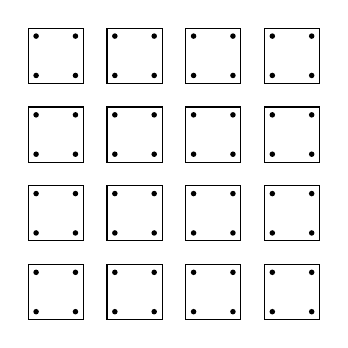
\begin{tikzpicture}[scale=0.5]
	\foreach \x in {0, ..., 7} 
	\foreach \y in {0, ..., 7} 
	{ 
		\fill (\x, \y) circle (2pt); 
	}
	\foreach \x in {0,..., 3}
	\foreach \y in {0,..., 3}  
	{ 
	\node [draw, thin, shape=rectangle, minimum width=0.7cm, minimum height=0.7cm, anchor=center] at (0.5 + 2 * \x, 0.5 + 2 * \y) {};
	}  
\end{tikzpicture}
	\qquad
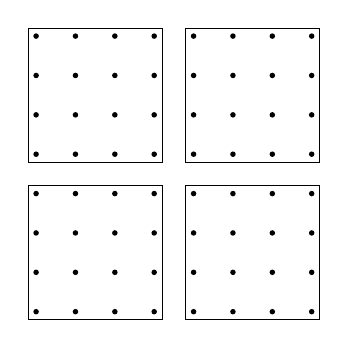
\begin{tikzpicture}[scale=0.5]
	\foreach \x in {0, ..., 7} 
	\foreach \y in {0, ..., 7} 
	{ 
		\fill (\x, \y) circle (2pt); 
	}
	\foreach \x in {0, 1} 
	\foreach \y in {0, 1} 
	{ 
			\node [draw, thin, shape=rectangle, minimum width=1.7cm, minimum height=1.7cm, anchor=center] at (1.5 + 4 * \x, 1.5 + 4 * \y) {};
	} 	  
\end{tikzpicture}
	
\caption{We can group up atoms to deal with less variables} 
	\label{fig:renormToy}  
\end{figure} 

This is shown in the first diagram. We've grouped atoms into sets of four, then we assign a single amalgamated value (like a spin average) to each group. Now, if this system exhibits \textbf{self similarity}, this means that in the new model, our structure of the Hamiltonian is the same, but our new parameters need to be changed to account for the grouping. So, our system is rewritten as \[ 
	H(J', B') = - J' \sum_{ \langle ij \rangle } \bar{s}_i \bar{s}_j  -  B' \sum_i \bar{ s}_i \]
So, by 'zooming' out of our system, we've mapped our pair of variables for from $(J, B) \rightarrow (J', B') $. This is the study of the renormalistion group. It explains universality because it predicts that different physical descriptors are just 'zoomed out' manifestations of other descriptors.  

Now, we can repeat this process even more and zoom out further, which will change the system even more. 
\subsubsection{Fixed points} 
Now, one may ask, what if we 'zoom out' according to procedures like the above, and observe the same behaviour. This is what is known as a fixed point. For example, if we had a magnetic system which is based on $T$, the temperature, and a coupling constant $J$, then if we take $T \rightarrow \infty, J = 0$, then we'll always see the same behavour of disorder no matter how much we zoom out. We'll touch on this in the later sections.

 
